\documentclass[11pt]{article}
\usepackage{graphicx}
\author{Ryan Smith \& David Cronkite \\ \{ryansmit, cronkd\}@uw.edu}
\title{Graded Reader}

\begin{document}
\maketitle

The goal of our app is to create a program that emulates a ``graded reader'' type book.  A graded reader is traditionally an L2 text that includes marginal notes and/or footnotes containing vocabulary the language learner is likely to have to look up in a dictionary at this stage in their studies. Its purpose is to provide the language learner with L2 texts to read without the frustration of having to constantly go back and forth between the text and a dictionary (especially if a dictionary might not help, as in a new grammar structure or an irregular word).  The ``graded'' part of graded reader implies a course-like structure going from very low level language ability, with large amounts of word definitions given, to a point where only a select few words need to have the translation given.

Our app will improve on this concept by allowing each word to be looked up when clicked, as in figure \ref{words}. Ideally, the file providing the text will include this definition in order to make it context sensitive. If it is not provided, the app will consult a dictionary. Even though the definition will be context insensitive, it will still give the user easy access to a dictionary entry.  Taking this a step further though, the user will also be able to select an entire sentence and have a translation provided for them (figure \ref{sentences}).  Again, the text provider will ideally provide the translations for contextual sensitivity. Otherwise, the app will use an external machine translation if possible.

\begin{figure}[h]
  \caption{Word definitions}
  \label{words}
  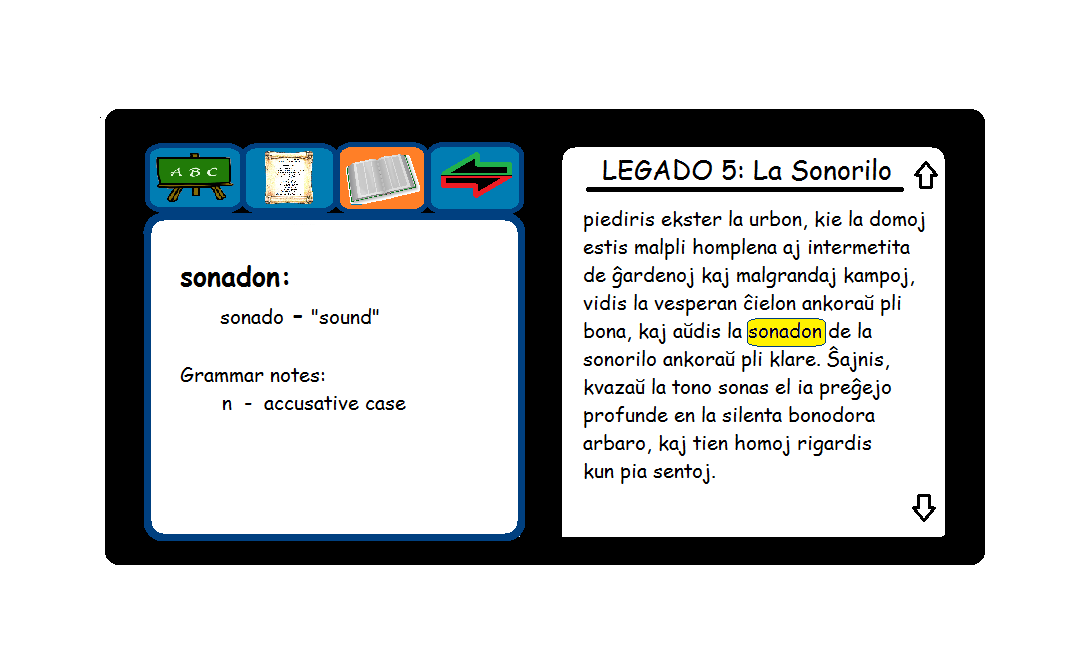
\includegraphics[scale=.5]{word_look_up.png}
\end{figure}

\begin{figure}[h]
  \caption{Sentence translation}
  \label{sentences}
  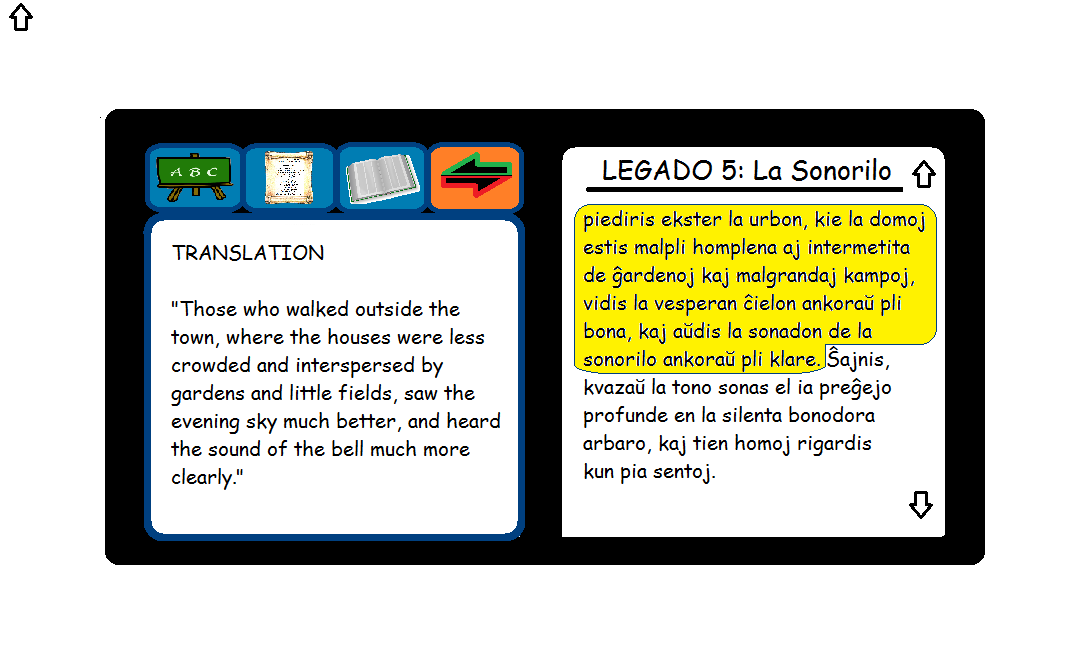
\includegraphics[scale=.5]{translate_tab.png}
\end{figure}

Besides just the dictionary look up, we will also include a list of ``most important vocabulary'' that provides the user with the words most likely needing to be looked up (see figure \ref{vocab}), just like a traditional graded reader would. This will allow the reader to not have to constantly click new words, as the text provider will already have included these problematic terms.

\begin{figure}[h]
  \caption{Vocabulary List}
  \label{vocab}
  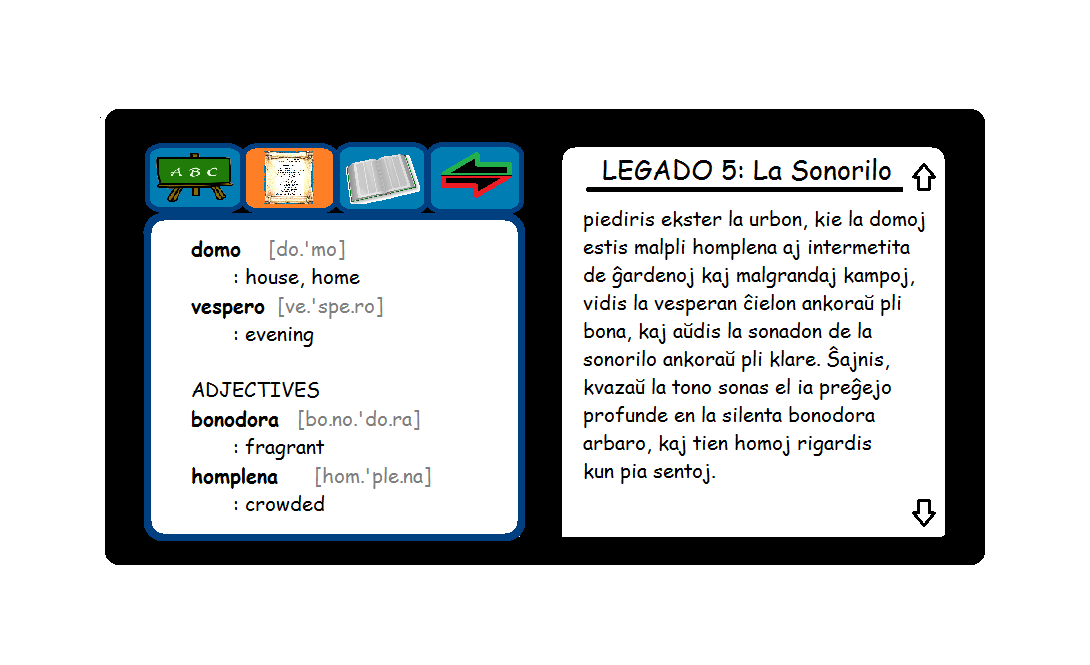
\includegraphics[scale=.5]{vocabulary_list.png}
\end{figure}

Further, we intend to include a section discussing new grammatical concepts, allowing our app to become a full language learning tool on its own. The user could peruse the new grammar before attempting to read the text in which the grammar concepts are found (figure \ref{grammar}).

\begin{figure}[h]
  \caption{New grammar information}
  \label{grammar}
  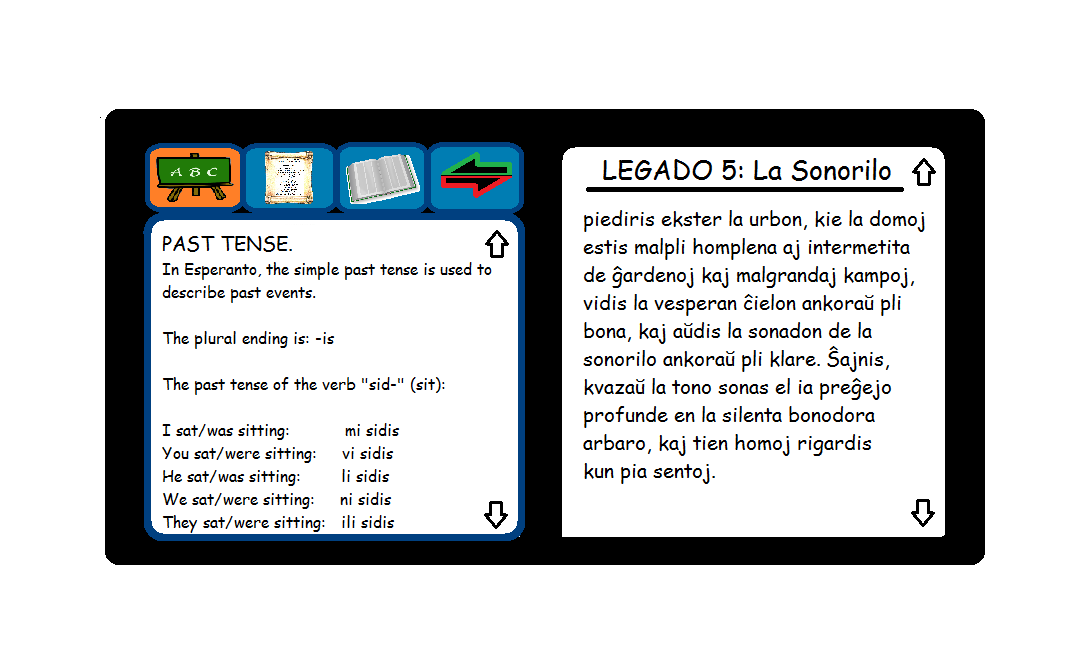
\includegraphics[scale=.5]{grammar_tab.png}
\end{figure}

While the SDK provides the main components we'll need (text views) in building this app, we will need to create the tabbed interface for the landscape view, as well as come up with some useful portrait views. In addition, we will need to create the linking between clicking on either a sentence or a word and have the appropriate translation appear in the window on the left.  We will also need the ability to do dictionary look ups and automatic translations for when the data file doesn't provide these. The data we'll need is texts which include information about the grammar, the new vocab, the context-sensitive word meanings, and possible sentence-level translations. We'll have to create these files ourselves, but the end goal is to create an open file format (probably XML) and a desktop application which anyone can use to generate new content.

\end{document}
